\section{Numerical evidence and separate error checks}
\label{sec:numerics}
The analysis establishes continuum optimal values. The computations
below serve two narrower purposes: they show how explicit designs
behave at finite budgets and examine the local uncertain-center
problem numerically. They use deterministic offset quadrature, not
sampling of tracer paths. No numerical value is assigned to
$\mathcal S_q$, and no discretized calculation is used to prove
the crossover theorem.

\subsection{Circle responses and exact discrete budget accounting}
By reflection symmetry we solve on $[0,\pi]$ with zero endpoint
flux and double the integrated response. With $n$ cells of width
$h=\pi/n$, cell centers $s_i=(i+1/2)h$, and nonnegative
face diffusivities $D_{i+1/2}$, the tridiagonal matrix is the
finite-volume discretization of
$-\partial_s(D\partial_s)+(c+\cos s)^2$. Its off-diagonal entry
is $-D_{i+1/2}/h^2$; its diagonal is the sum of adjoining
conductances plus the midpoint reaction. We solve against the
vector of ones and approximate $J_c$ by $2h\sum_i h_i$.
There are no faces beyond the two endpoints.
Every compared field, including the uniform field, is normalized
to the same discrete budget
\[
                   2h\sum_{i=1}^{n-1}D_i=M.
\]
This normalization tends to the continuum integral constraint as
the mesh is refined. It is necessary when sampling a singular or
concentrated continuum shape; otherwise finite-grid comparisons
would use slightly different resources.

The predetermined mean trial samples $|\sin s|^{-2/5}$. This
integrable unrounded shape has the same leading mean coefficient
as \eqref{eq:sharp-subcritical-design}: it bounds the rounded
profile from below by a multiplicative factor tending to one,
so monotonicity and the sharp lower bound squeeze its leading
cost to $K_1M^{-1/4}$. For $q=8/5$ and $q=3$, we use the
distance-based graded field \eqref{eq:graded-design} with
\eqref{eq:graded-cutoffs}, evaluated with its exact continuum
normalization before imposing the discrete mass above.
At criticality its leading coefficient is also $K_{\rm crit}$:
distance and $|\sin s|$ have ratio tending to one near either
fold, their normalization integrals both equal
$4\log(1/R)+O(1)$, and the leading logarithmic contribution
comes from those fold approaches.
More explicitly, on the retained annuli
$R\log(1/M)\le r\le r_*$, with fixed small $r_*>0$,
$(r+R)/(|\sin r|+R)=1+O(r_*^2)$. The part $r\ge r_*$
has critical moment $O(a_R^{-2/5})$, one logarithmic factor
smaller than the leading contribution. The inner omitted annuli
obey the same bounds as in the critical proof of
\cref{thm:blind-sharp}. First let $M\to0$ and then
$r_*\to0$ to obtain the stated coefficient.
The $q=3$ field is an
order-optimal trial; its scaled cost is not identified with
$2^{(33-12)/7}\mathcal S_3$.

We also evaluate a simple exact-observation trial to illustrate
finite-budget performance. For $0\le c<1$, put
$r=\arccos(-c)$, $a=1-c^2$, and
$R=(40M/(3a))^{1/5}$. If
$R<0.3\min(r,\pi-r)$, use the quadratic profile
\eqref{eq:placement-profile} centered at $r$ on the half-wall.
Otherwise use a constant patch adjacent to $\pi$ of extent
\[
          E=\min\{\pi,\max(4M^{1/7},2(\pi-r))\}.
\]
The full-wall field is its reflection; in the continuum the
patch value is $M/(2E)$. For $c\ge1$ use uniform mobility,
and extend the policy to negative $c$ by translation by $\pi$.
The discrete normalization is applied to each realization.
This is an evaluated trial, distinct from the policy used for
the sharp asymptotic proof in \cref{sec:exact-observation}.
Its finite-budget values do not certify the exact-observation
optimum.

For these symmetric fields the ensemble moment is
$(1/2)\int_0^2 J_c^q\dd c$. We subdivide this interval at
$0,0.5,0.9,1,1.1,1.5,2$ and at the valid points
$1\pm\lambda w$, with $\lambda=0.1,1,10,100$ and
$w$ drawn from the squared grading radius,
$(M/(4\pi))^{1/3}$, and $M^{2/7}$. For the unrounded $q=1$
trial the first of these subdivision widths is also set to
$M^{2/7}$; it is a quadrature scale, not a profile cutoff.
Duplicate and out-of-range
points are removed. Each subinterval uses Gauss--Legendre
quadrature. The main computations have $n=32768$ and 48 nodes
per subinterval. Both the full list of subdivisions and the
unscaled ensemble moments are supplied with the data.

\begin{figure}[t]
\centering
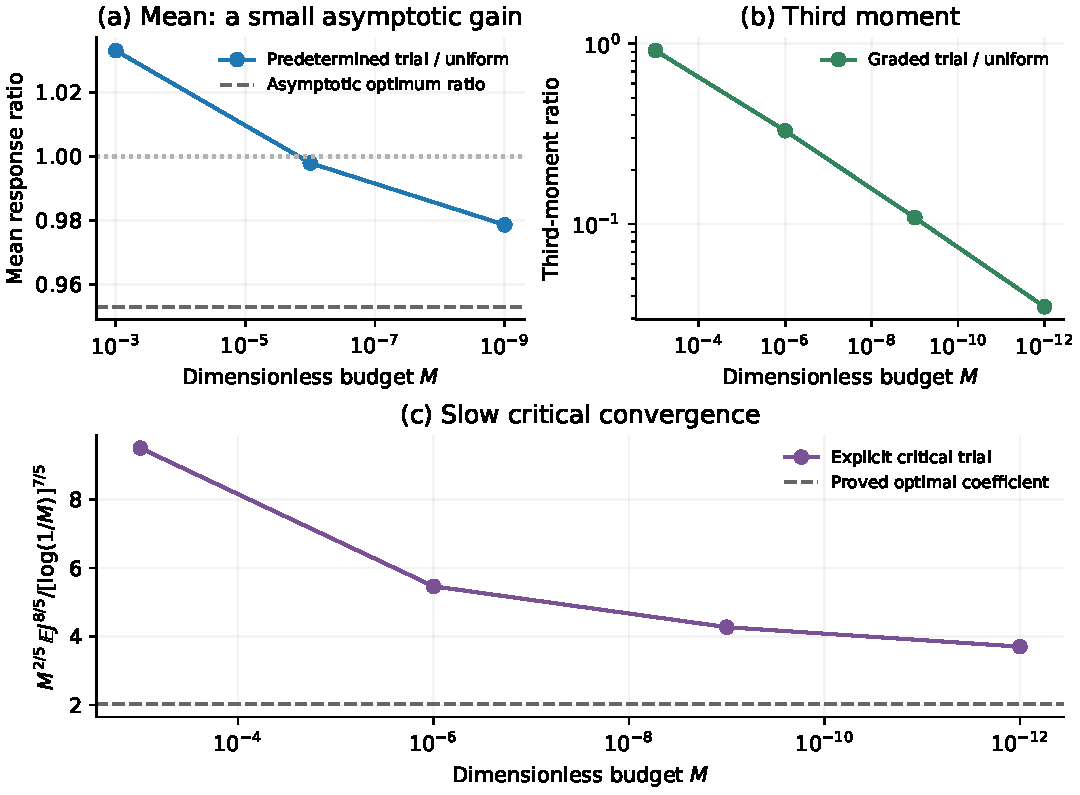
\includegraphics[width=\textwidth]{figures/moment-designs.pdf}
\caption{Finite-volume evaluation of explicit mobility trials, with the
same discrete budget for each field. (a) A mean-optimal asymptotic shape
can be worse than the uniform field at finite budget. (b) Grading has a
larger effect on the third moment. (c) The critical scaled trial cost
converges slowly toward the proved optimal coefficient. Curves are
trial evaluations, not finite-budget optimal values; the dashed
coefficients are continuum asymptotic results.}
\label{fig:moment-designs}
\end{figure}

\Cref{fig:moment-designs,tab:mean-trials} show the finite-budget
distinction. The predetermined trial is about $3.3\%$ worse than
uniform mobility at $M=10^{-3}$, despite its smaller asymptotic
coefficient: the limiting ratio is
$K_1/[C_0^2(2\pi)^{1/4}/\sqrt\pi]=0.9529814\ldots$.
At $M=10^{-9}$ its numerical improvement is only about $2.1\%$.
The observed trial yields a larger improvement, but its ratio
to the predetermined trial is not the ratio of their finite-budget
optima. For the third moment the graded-to-uniform ratio decreases
from about $0.914$ at $10^{-3}$ to $0.0348$ at $10^{-12}$.
At the critical order, the scaled trial moment decreases from
$9.495$ to $3.702$ over that budget range, still well above
$K_{\rm crit}=2.02233076\ldots$.

\begin{table}[t]
\centering
\caption{Mean response ratios from the main circle computations.
Both columns concern explicitly evaluated fields, with no numerical
optimization over circle coefficients.}
\label{tab:mean-trials}
\begin{tabular}{@{}ccc@{}}
\toprule
$M$ & Predetermined trial / uniform & Observed trial / predetermined trial\\
\midrule
$10^{-3}$ & 1.0331 & 0.8269 \\
$10^{-6}$ & 0.9980 & 0.5942 \\
$10^{-9}$ & 0.9786 & 0.4297 \\
\bottomrule

\end{tabular}
\end{table}

We refine space and offset quadrature separately at the smallest
budget for each of $q=1,8/5,3$. Doubling the half-wall grid to
65536 cells at fixed 48-node quadrature changes the predetermined
mean trial, critical moment trial, and third-moment trial by
$0.0158\%$, $0.0084\%$, and $0.1184\%$, respectively, in absolute
relative terms. Doubling the quadrature to 96 nodes at the original
grid changes those three quantities by less than $10^{-8}$ relative.
The discontinuous observed-trial branch selection gives a larger,
but still small, quadrature change of $6.5\times10^{-6}$ at
$M=10^{-9}$. A combined 65536-cell, 96-node calculation is also
included. These checks assess stability of the reported trial
values; they are not rigorous continuum error bounds or a test of
the full bulk--surface model.

\subsection{The local uncertain-center problem}
For \eqref{eq:center-value}, restrict mobility to $[-L,L]$ with
$L=6+\eta/2$. Use $n$ cells of width $h=2L/n$ and optimize the
nonnegative interior face masses $p_i=hD_i$, with $\sum_i p_i=1$.
The reaction at cell center $x_j$ for a center $z$ is
$(x_j-z)^2$, and face conductance is $p_i/h^3$.
The interior problem has zero endpoint flux. Mobility is exactly
zero outside the interval, so its exterior response is added
analytically. Its averaged value is
\begin{equation}\label{eq:numeric-exterior}
 \frac2\eta\log\frac{L+\eta/2}{L-\eta/2}\quad(\eta>0),
       \qquad \frac2L\quad(\eta=0).
\end{equation}
There is therefore no omitted reciprocal-potential tail; the
remaining domain restriction is on where mobility can be placed.
For $\eta>0$ the center average uses Gauss--Legendre quadrature
on $[-\eta/2,\eta/2]$.

We minimize this convex discrete objective $F_h(p)$ by sequential
least squares programming, starting from uniform face masses and
using the exact matrix derivative. If $h_z$ denotes the solved
source vector, that derivative is
\[
       g_i=\partial_{p_i}F_h
           =-\sum_z w_z\left(\frac{h_{z,i+1}-h_{z,i}}h\right)^2.
\]
For any feasible returned vector $p$, convexity gives the global
discrete bounds
\begin{equation}\label{eq:numeric-tangent}
        F_h(p)-\delta_h\le\inf_{r_i\ge0,\,\sum r_i=1}F_h(r)
                     \le F_h(p),\qquad
        \delta_h=g\cdot p-\min_i g_i.
\end{equation}
Negligible feasibility error is projected onto the simplex before
evaluating these quantities. The formula is an analytical certificate
for the discretized problem, evaluated in floating-point arithmetic.
It neither bounds continuum discretization error nor provides
interval-certified arithmetic.

\begin{table}[t]
\centering
\caption{Uncertain-center discrete values with 400 cells. Center
quadrature has 96 nodes at $\eta=2,8$, 192 at $\eta=32$, and one
known center at zero. The lower value and gap use
\eqref{eq:numeric-tangent} for the same finite-dimensional objective.}
\label{tab:center-values}
\begin{tabular}{@{}rrrr@{}}
\toprule
$\eta$ & Computed value & Discrete tangent lower value & Gap $\delta_h$\\
\midrule
0 & 6.222655 & 6.220971 & 0.0017 \\
2 & 6.633100 & 6.630905 & 0.0022 \\
8 & 8.082211 & 8.081774 & 0.00044 \\
32 & 11.138582 & 11.138439 & 0.00014 \\
\bottomrule

\end{tabular}
\end{table}

\begin{figure}[t]
\centering
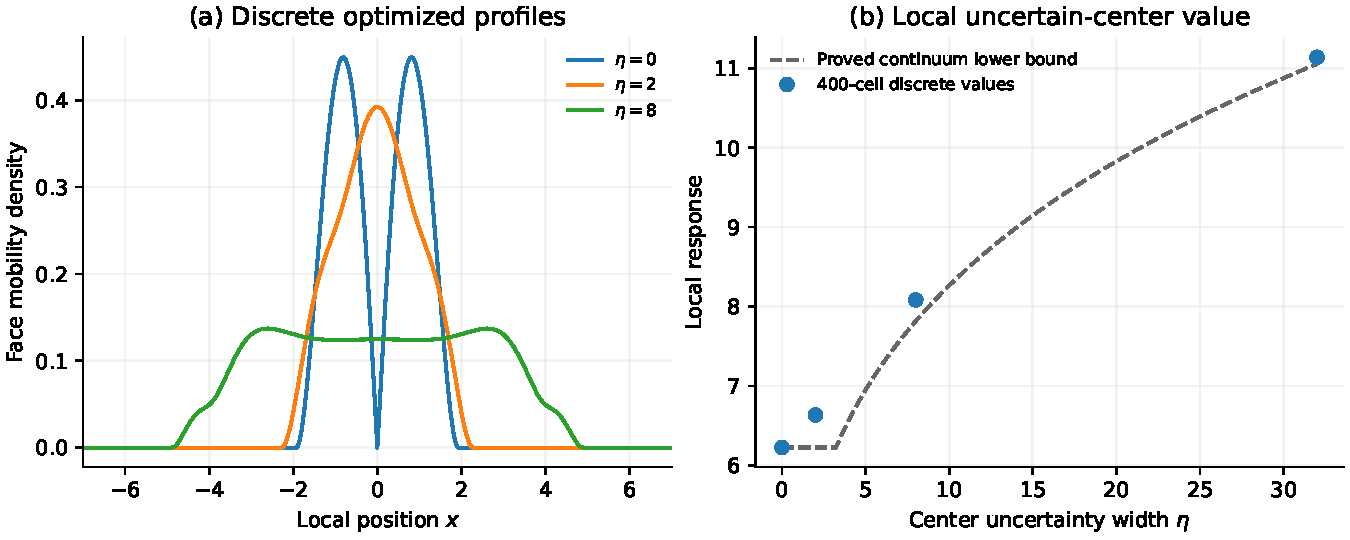
\includegraphics[width=.95\textwidth]{figures/uncertain-center.pdf}
\caption{Finite-dimensional optimization of the local uncertain-center
problem. (a) Optimized face profiles broaden as center uncertainty
increases in the displayed examples. (b) Discrete computed values
and the proved continuum bound
$\max(C_{\rm pl},C_0\eta^{1/4})$. The discrete markers have
discretization error and are not certified continuum upper bounds.
Neither the figure nor the theorem asserts monotonicity of all
minimizing profiles.}
\label{fig:uncertain-center}
\end{figure}

\Cref{tab:center-values,fig:uncertain-center} show the 400-cell
calculations. At $\eta=0$ the computed value $6.222655$ lies
slightly below the exact continuum value
$C_{\rm pl}=6.222823736\ldots$, illustrating why a discrete
tangent interval must not be read as a continuum interval.
Increasing the grid from 200 to 400 cells changes the objective
by about $0.0082\%$, $0.0136\%$, and $0.518\%$ at
$\eta=0,2,32$, respectively. At $\eta=0,2$, these changes are smaller
than the remaining discrete optimization uncertainty. They show
stability of the returned objective values but do not separately
resolve spatial discretization error. Re-evaluating every 400-cell field
on 384 center nodes changes the objective by less than
$10^{-12}$ relative. At $\eta=32$, enlarging $L$ from 22 to 33
while keeping $h=0.11$ (400 to 600 cells) changes the computed
value by $6.8\times10^{-8}$ relative. This domain check concerns
the computed value; its difference is smaller than the discrete
optimization gaps and is not an independent rigorous tail bound.

A deliberately underresolved parameter calculation exposes a
different error. At $\eta=32$, optimizing 200 cells on only 24
center nodes gives $10.84053$ with a small discrete tangent gap.
Re-evaluating that same field on 384 nodes gives $12.09482$, an
increase of about $11.6\%$. A small optimization gap can therefore
certify an overfitted quadrature problem. Spatial refinement,
independent parameter quadrature, and optimization error must be
checked separately. The continuum claims remain the exact
variational characterizations and proved limits, not decimal
values inferred from these finite grids.

\subsection{Reproducibility}
The accompanying \texttt{numerics/reproduce.py} regenerates the
data, both figures, and the numerical table rows. The saved
\texttt{data/numerical-evidence.json} includes every grid size,
quadrature subdivision, feasibility check, optimizer status,
tangent gap, and refinement used above. The script requires
Python, NumPy, SciPy, and Matplotlib and imports the documented
tridiagonal circle solver and graded trial construction from the
repository's \texttt{scripts} directory. The folder README gives
the exact commands and environment versions. Figures and tables
are included in the manuscript source so that LaTeX compilation
does not require rerunning the numerical optimization.
